\documentclass[11pt,a4paper]{article}
\usepackage{amsmath,amssymb}
\usepackage{enumitem}
\setlength{\parindent}{0pt}
\setlength{\parskip}{0.55em}
\sloppy
\usepackage[spanish,es-tabla]{babel}
\usepackage[utf8]{inputenc}
\usepackage[T1]{fontenc}
\usepackage{graphicx}
\usepackage{xcolor}
\usepackage{pdfpages}
\usepackage{geometry}
\usepackage{hyperref}
\usepackage{array}
\usepackage[protrusion=true,expansion=false]{microtype}
\usepackage{tikz}
\usepackage{multicol}
\geometry{margin=2cm}
\definecolor{sincblue}{HTML}{1E73BE}
\definecolor{sincpurple}{HTML}{6D38B8}
\hypersetup{colorlinks=true, linkcolor=sincblue, urlcolor=sincblue}
%
%\newcommand{\sincpagenumber}{%
%  \thispagestyle{empty}%
%  \begin{tikzpicture}[remember picture,overlay]
%    % Parche blanco para tapar el número original del PDF
%    \fill[white]
%      ([xshift=-2.5cm,yshift=0.55cm]current page.south)
%      rectangle
%      ([xshift=2.5cm,yshift=1.35cm]current page.south);
%
%    % Nuevo número de página centrado
%    \node[font=\normalfont\normalsize]
%      at ([yshift=0.95cm]current page.south) {\thepage};
%  \end{tikzpicture}%
%}


\begin{document}

%\begin{titlepage}
%\centering
%\vspace*{0.5cm}
%
\includegraphics[width=.72\textwidth]{assets/SINC_LOGO.png}\\[.8cm]

%{\Huge \textbf{Libro de abstracts}\\[2.4cm]}
%{\Huge\bfseries SINC II\\[.2cm]}
%{\Large Simposio de Investigadores Noveles en Complejidad\\[.8cm]}

%{\large Universidad Rey Juan Carlos -- 02/06/2026}\\[1cm]
%
\includegraphics[width=.38\textwidth]{assets/URJC.jpg}
%\end{titlepage}



\begin{titlepage}

\thispagestyle{empty}
\begin{center}

% Logo principal
{\vspace{-3cm}
\includegraphics[ width=.65\textwidth]{assets/SINC_LOGO.png}
}

{\vspace{-1cm}\fontsize{20}{36}\selectfont \bfseries SINC II\par}

{\huge $2^{a}$ Edici\'on del Simposio de Investigadores Noveles en Complejidad\par}

% Título principal
\rule{0.95\textwidth}{0.4pt}

{\fontsize{25}{36}\selectfont \bfseries Libro de resúmenes\par}

\rule{0.95\textwidth}{0.4pt}


\vspace{1.5cm}

{\huge
Universidad Rey Juan Carlos\\[0.2cm]
\par}

{\Large
12 de junio de 2026
\par}



\vfill

\vspace{0.8cm}

% Logo institucional

\includegraphics[width=.30\textwidth]{assets/URJC.jpg}\hspace{3cm}

\includegraphics[width=.45\textwidth]{assets/ESCET.png}


\vspace{0.6cm}

\end{center}
\end{titlepage}








\clearpage
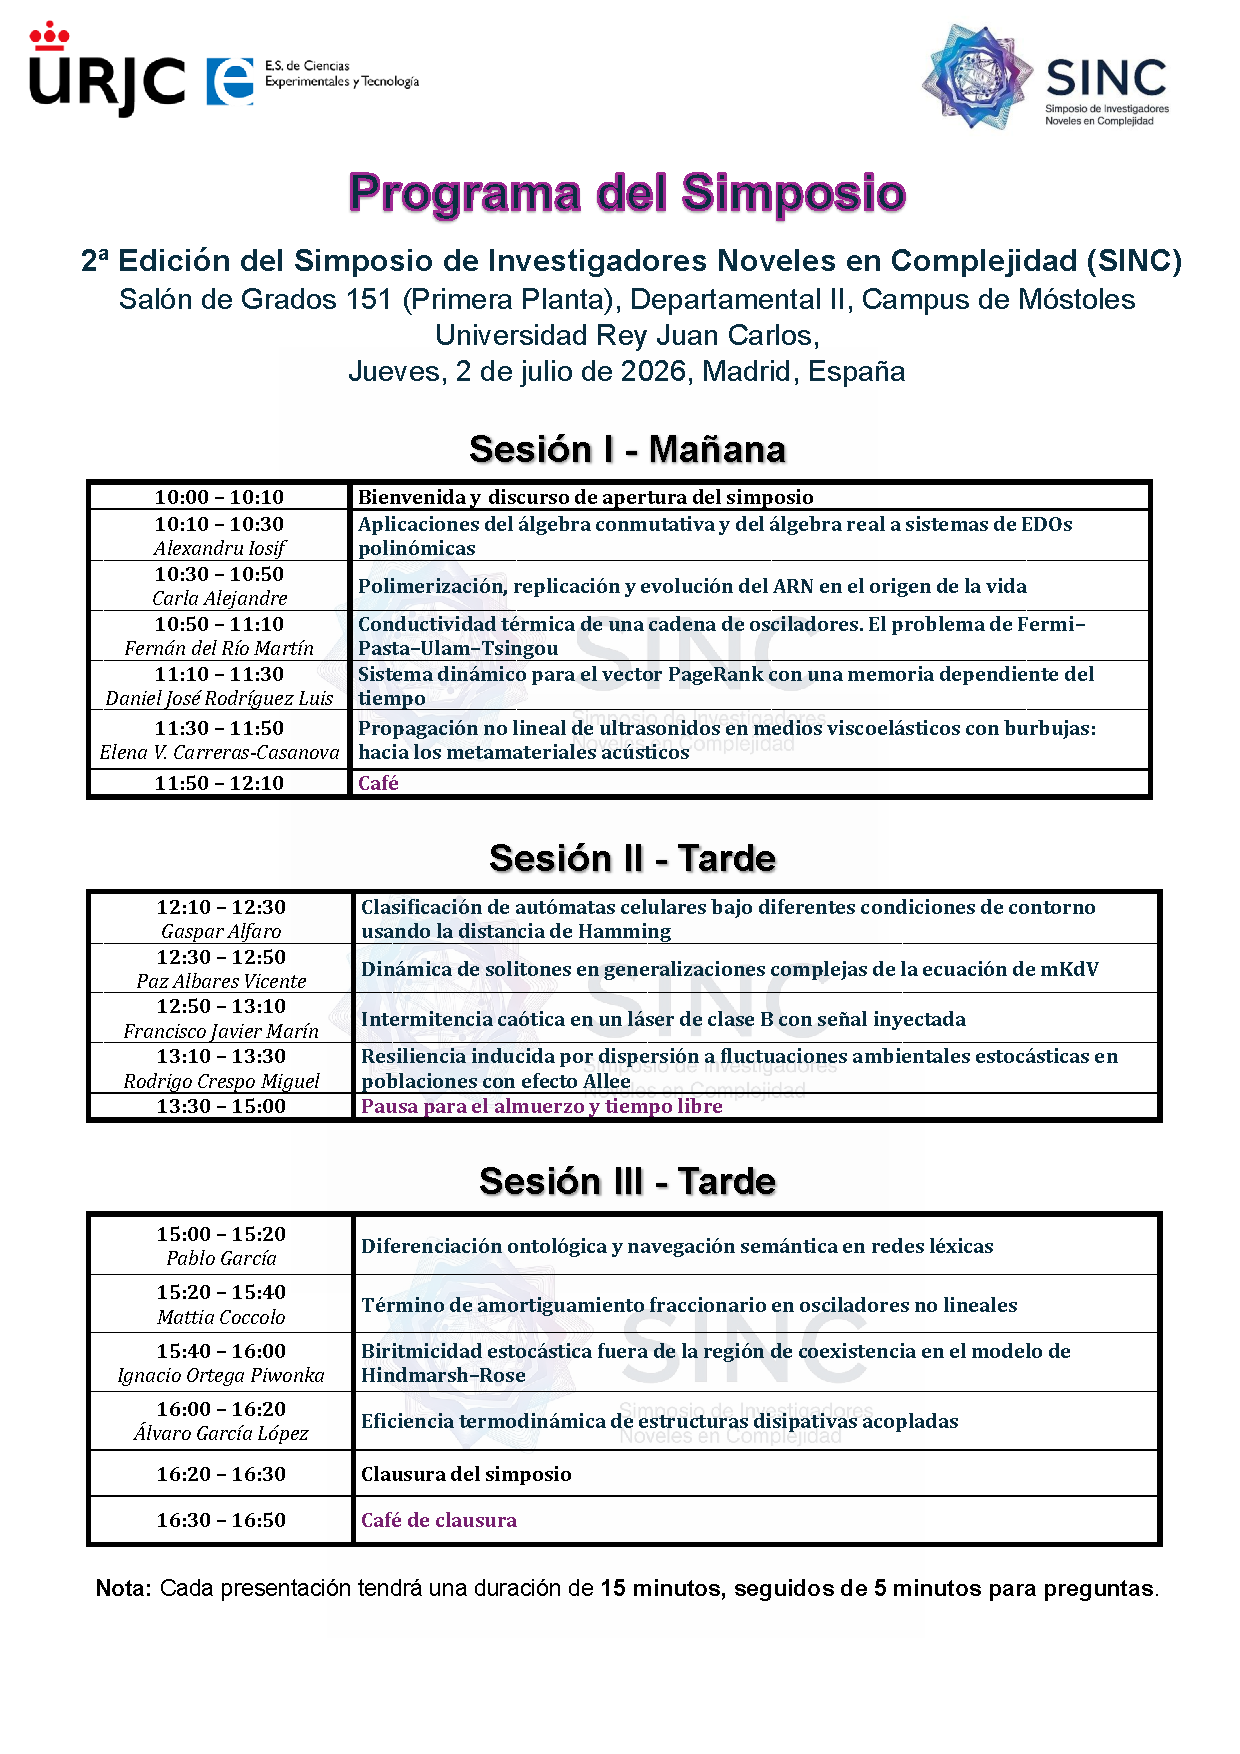
\includepdf[pages=-,pagecommand={\thispagestyle{plain}}]{Programa_SINC_2026.pdf}
\clearpage

\clearpage
\phantomsection
\addcontentsline{toc}{section}{Introducción}

\thispagestyle{plain}

\vspace*{1.0cm}

\begin{center}
    {\Huge\bfseries Introducción}
\end{center}

\vspace*{2.5cm}

\begin{center}
\begin{minipage}{0.82\textwidth}
\large

El Simposio de Investigadores Noveles en Complejidad (SINC) celebra en esta edición su segundo encuentro, consolidándose como un espacio de intercambio científico dentro de la Universidad Rey Juan Carlos. El objetivo principal del simposio es reunir a investigadores jóvenes —y también a quienes, sin serlo ya tanto, mantienen intacta la curiosidad científica— para compartir líneas de trabajo, conocer la investigación que se desarrolla en distintas áreas de la universidad y favorecer posibles colaboraciones futuras.

\vspace{0.7em}

Aunque el nombre del simposio está inspirado en el ámbito de los sistemas no lineales, la complejidad y la sincronización, SINC nace con una vocación amplia e interdisciplinar. Por ello, esta edición acoge contribuciones procedentes de diferentes campos científicos, con el propósito de fomentar el diálogo entre áreas, identificar puntos de contacto entre metodologías y problemas diversos, y reforzar la comunidad investigadora de la URJC.

\vspace{0.7em}

Este libro recoge los resúmenes de las contribuciones presentadas en SINC II. Más que un simple registro de comunicaciones, pretende ser una pequeña muestra de la variedad, calidad y vitalidad de la investigación desarrollada por investigadores e investigadoras vinculados a la Universidad Rey Juan Carlos y a su entorno científico.

\vspace{1.4em}

{\normalsize
\noindent\textbf{Licencia.} Este libro de abstracts se distribuye bajo la licencia Creative Commons Attribution-NonCommercial-NoDerivatives 4.0 International (CC BY-NC-ND 4.0), salvo indicación contraria. Los derechos de cada resumen pertenecen a sus respectivos autores.
}

\vspace{2.0cm}

{
\Large
12 de julio de 2026
\par}

\vspace{0.4cm}

{\large
\textbf{DOI:}
\href{https://doi.org/10.5281/zenodo.20668842}
     {10.5281/zenodo.20668842}
\par}

\end{minipage}
\end{center}

\vfill

\clearpage


%\section*{Nota editorial provisional}
%Este documento es una primera maqueta del libro de abstracts del SINC II. Se ha preparado a partir de los archivos recibidos, conservando los PDFs originales cuando estaban disponibles e incorporando la versión actualizada del abstract de Mattia Coccolo con sus referencias.
%
%Se ha dejado fuera provisionalmente el archivo de Pablo García, porque contiene un manuscrito/artículo de 17 páginas y no un abstract breve. También se ha descartado la versión inglesa duplicada del abstract de Ignacio Ortega Piwonka, conservando la versión en español.

\begin{center}
\section*{\Huge Índice}
\end{center}

\thispagestyle{plain}

\vspace*{1.00cm}
%\vfill

\begin{center}
\begin{minipage}{0.9\textwidth}
\large
\begin{enumerate}
  \item \textbf{Aplicaciones del álgebra conmutativa y del álgebra real a sistemas de EDOs polinómicas} \\ \emph{Alexandru Iosif} \dotfill \ \hspace{0.1cm} \pageref{abs:1}

  \item \textbf{Polimerización, replicación y evolución del ARN en el origen de la vida} \\ \emph{Carla Alejandre} \dotfill \ \hspace{0.1cm} \pageref{abs:2}

  \item \textbf{Sistema dinámico para el vector PageRank con una memoria dependiente del tiempo} \\ \emph{Daniel José Rodríguez Luis} \dotfill \ \hspace{0.1cm} \pageref{abs:3}

  \item \textbf{Propagación no lineal de ultrasonidos en medios viscoelásticos con burbujas: hacia los metamateriales acústicos} \\ \emph{Elena V. Carreras-Casanova} \dotfill \ \hspace{0.1cm} \pageref{abs:4}

  \item \textbf{Conductividad térmica de una cadena de osciladores. El problema de Fermi-Pasta-Ulam-Tsingou} \\ \emph{Fernán Del Río Martín} \dotfill \ \hspace{0.1cm} \pageref{abs:5}

  \item \textbf{Intermitencia caótica en un láser de clase B con señal inyectada} \\ \emph{Francisco Javier Marín Rodríguez} \dotfill \ \hspace{0.1cm} \pageref{abs:6}

  \item \textbf{Clasificación de autómatas celulares bajo diferentes condiciones de contorno usando la distancia de Hamming} \\ \emph{Gaspar Alfaro} \dotfill \ \hspace{0.1cm} \pageref{abs:7}

  \item \textbf{Biritmicidad estocástica fuera de la región de coexistencia en el modelo de Hindmarsh-Rose} \\ \emph{Ignacio Ortega Piwonka} \dotfill \ \hspace{0.1cm} \pageref{abs:8}

  \item \textbf{Término de amortiguamiento fraccionario en osciladores no lineales} \\ \emph{Mattia Coccolo} \dotfill \ \hspace{0.1cm} \pageref{abs:9}

  \item \textbf{Diferenciación ontológica y navegación semántica en redes léxicas} \\ \emph{Pablo García} \dotfill \ \hspace{0.1cm} \pageref{abs:10}

  \item \textbf{Dinámica de solitones en generalizaciones complejas de la ecuación de mKdV} \\ \emph{Paz Albares Vicente} \dotfill \ \hspace{0.1cm} \pageref{abs:11}

  \item \textbf{Resiliencia inducida por dispersión a fluctuaciones ambientales estocásticas en poblaciones con efecto Allee} \\ \emph{Rodrigo Crespo Miguel} \dotfill \ \hspace{0.1cm} \pageref{abs:12}

  \item \textbf{Eficiencia termodinámica de estructuras disipativas acopladas} \\ \emph{Álvaro García López} \dotfill \ \hspace{0.1cm} \pageref{abs:13}

\end{enumerate}


\vspace{0.1cm}
\hrule
\vspace{0.1cm}

\hspace*{+0.95cm}%
\textbf{Temas tratados}
\dotfill
\pageref{sec:temas}

\medskip

\hspace*{+0.95cm}%
\textbf{Ponentes y particpantes}
\dotfill
\pageref{sec:ponentes}

\medskip

\hspace*{+0.95cm}%
\textbf{Comité organizador}
\dotfill
\pageref{sec:comite}



\end{minipage}
\end{center}



% -----------------------------------------------------------------------------
% Abstracts remaquetados para SINC II
% Copiar este bloque antes de \end{document}.
% Requiere en el preámbulo:
%   \usepackage{amsmath,amssymb}
%   \usepackage{enumitem}
% Opcional:
%   \sloppy
% -----------------------------------------------------------------------------

\newcommand{\sincAbstractPage}[2]{%
\clearpage
\phantomsection
\addcontentsline{toc}{section}{#2}
\label{abs:#1}
\thispagestyle{plain}

\begin{tikzpicture}[remember picture,overlay]
    \node[anchor=south east]
    at ([xshift=-11.8cm,yshift=27.2cm]current page.south east)
    {
\includegraphics[width=9cm]{assets/urjc_escet.png} };
\end{tikzpicture}
\begin{tikzpicture}[remember picture,overlay]
    \node[anchor=south east]
    at ([xshift=-1.cm,yshift=25.6cm]current page.south east)
    {
\includegraphics[width=4.8cm]{assets/SINC_LOGO.png} };
\end{tikzpicture}

\vspace*{.5cm}

\begin{center}
    {\LARGE\bfseries Contribución #1} \\
\end{center}

%\vfill

%\begin{center}
%    {\LARGE\bfseries #2}
%\end{center}

%\vfill
%\clearpage
}
\newenvironment{sincabstract}[4]{%
\begin{center}
{\Large\bfseries #1\par}
\vspace{0.6cm}
{\normalsize #2\par}
{\small #3\par}
{\small\texttt{#4}\par}
\end{center}
\vspace{0.4cm}
}{%
\clearpage
}

\newcommand{\keywords}[1]{\vspace{0.4cm}\noindent\textbf{Palabras clave:} #1}
\newcommand{\keywordsEN}[1]{\vspace{0.4cm}\noindent\textbf{Keywords:} #1}

% -----------------------------------------------------------------------------
% ABSTRACT 1
% -----------------------------------------------------------------------------
\sincAbstractPage{1}{Aplicaciones del álgebra conmutativa y del álgebra real a sistemas de EDOs polinómicas}

\begin{sincabstract}
{Aplicaciones del álgebra conmutativa y del álgebra real a sistemas de EDOs polinómicas}
{Alexandru Iosif\textsuperscript{1}}
{\textsuperscript{1} Área de Matemática Aplicada de la Universidad Rey Juan Carlos}
{alexandru.iosif@urjc.es}

\paragraph{Resumen.}
Considérese una familia de sistemas de EDOs de primer orden,
\begin{equation*}
\begin{cases}
\dot{x}_1 = P_1(k_1,\ldots,k_m;x_1,\ldots,x_n),\\
\vdots\\
\dot{x}_n = P_n(k_1,\ldots,k_m;x_1,\ldots,x_n),
\end{cases}
\end{equation*}
donde $P_i$ son funciones polinómicas en las funciones $x_1,\ldots,x_n$ y racionales en los parámetros $k_1,\ldots,k_m$. En esta breve charla pretendemos hacer una introducción a los métodos algebraicos para el estudio de estos sistemas. En particular, vamos a mostrar cómo las bases de Gröbner, la eliminación de cuantificadores, los discriminantes y las sizigias, entre otras herramientas, sirven para la clasificación de los puntos estacionarios, de primeras integrales, etc. en dichos sistemas. Finalmente, mostramos algunas aplicaciones a redes moleculares.

\keywords{reducción de la complejidad, dinámica no lineal, álgebra aplicada y computacional.}

\begin{multicols}{2}
\begin{enumerate}[label={[\arabic*]},leftmargin=*]
\item A. Iosif, Duality in mass-action networks, Preprint (2026).
\item A. Desoeuvres, A. Iosif, C. Lüders, O. Radulescu, H. Rahkooy, M. Seiß, T. Sturm, A Computational Approach to Polynomial Conservation Laws, \textit{SIAM Journal on Applied Dynamical Systems} 23(1), (2024).
\item A. Desoeuvres, A. Iosif, C. Lüders, O. Radulescu, H. Rahkooy, M. Seiß, T. Sturm, Reduction of Chemical Reaction Networks with Approximate Conservation Laws, \textit{SIAM Journal on Applied Dynamical Systems} 23(1) (2024).
\item D. Grigoriev, A. Iosif, H. Rahkooy, T. Sturm, A. Weber, Efficiently and Effectively Recognizing Toricity of Steady State Varieties, \textit{Mathematics in Computer Science} 15 (2020).
\item C. Conradi, A. Iosif, and T. Kahle, Multistationarity in the space of total concentrations for systems that admit a monomial parametrization, \textit{Bulletin of Mathematical Biology} 81(10) (2019).
\item A. Iosif, Algebraic Methods for detecting multistationarity in mass-action network, PhD Thesis, Otto-von-Guericke Universität, 2019.
\end{enumerate}

\end{multicols}
\end{sincabstract}

% -----------------------------------------------------------------------------
% ABSTRACT 2
% -----------------------------------------------------------------------------
\sincAbstractPage{2}{Polimerización, replicación y evolución del ARN en el origen de la vida}

\begin{sincabstract}
{Polimerización, replicación y evolución del ARN en el origen de la vida}
{Carla Alejandre\textsuperscript{1,2}, Carlos Briones\textsuperscript{1}, Jacobo Aguirre\textsuperscript{1,2}}
{\textsuperscript{1} Centro de Astrobiología (CAB), CSIC-INTA, Torrejón de Ardoz, Madrid, España\\
\textsuperscript{2} Grupo Interdisciplinar de Sistemas Complejos (GISC), Madrid, España}
{calejandre@cab.inta-csic.es}

\vspace{-0.5cm}

\paragraph{Resumen.}
Cómo surgió la vida a partir de materia no viva hace aproximadamente 4 mil millones de años es una de las preguntas abiertas más profundas de la ciencia. Dado que la evidencia empírica directa de la Tierra primitiva es escasa, este problema resulta especialmente adecuado para su exploración teórica y computacional. En nuestra investigación abordamos este desafío desde una perspectiva de sistemas, centrándonos en el aumento abrupto de complejidad que se produjo cuando aparecieron las primeras moléculas de ARN y comenzaron a experimentar evolución darwiniana. El ARN es el único biopolímero natural conocido capaz de codificar información genética y, al mismo tiempo, desempeñar funciones catalíticas, acoplando de forma efectiva genotipo y fenotipo dentro de un único marco molecular. Esta propiedad constituye la base de la hipótesis del mundo de ARN [1]. Sin embargo, sigue siendo un reto comprender cómo pudieron surgir los primeros polímeros de ARN y cómo pudieron replicarse y evolucionar posteriormente en la Tierra primitiva, en ausencia de enzimas complejas e incluso de mecanismos de replicación precisos. Hemos desarrollado un marco teórico y computacional denominado EarlyWorld. Este modelo se utilizó inicialmente para demostrar que la polimerización no enzimática de ribonucleótidos y la replicación dependiente de molde de polímeros de ARN, suficientemente largos como para plegarse y adquirir funciones básicas ($>15$ nt), eran factibles en interfaces arcilla-agua en la Tierra prebiótica [2]. El requisito esencial es que el entorno físico-químico estuviera caracterizado por oscilaciones de gran amplitud con una periodicidad compatible con la dinámica de las mareas vivas. Actualmente estamos aplicando EarlyWorld al estudio del potencial evolutivo de los polímeros primordiales de ARN. Considerando tanto factores de selección ambientales como internos, e incorporando los efectos de los fenotipos de ARN sobre su propia replicación, buscamos esclarecer si la complejificación, la selección y, en última instancia, la evolución del ARN en la Tierra prebiótica pudieron ser posibles a partir de un sistema basado únicamente en mecanismos aleatorios y de ligación dependiente de molde.
%\enlargethispage{1.75\baselineskip}

\begin{multicols}{2}

\begin{center}
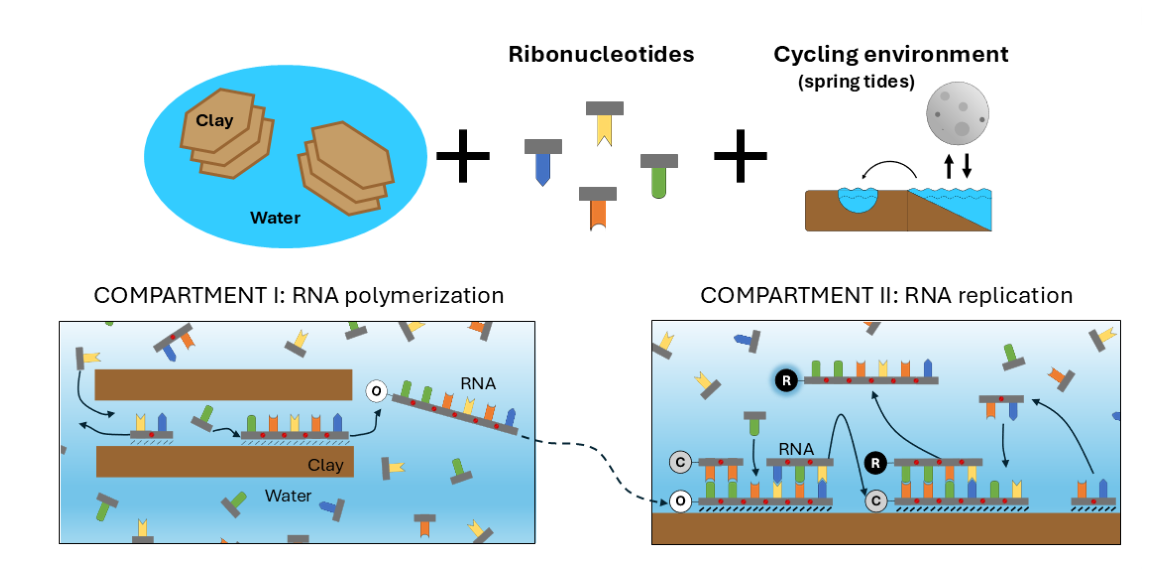
\includegraphics[width=0.48\textwidth]{figures/carla_alejandre_fig01_p1_crop.png}


{\small Figura 1. Esquema conceptual del marco EarlyWorld para la polimerización, replicación y evolución del ARN en el origen de la vida.}
\end{center}
\vspace{-1.8em}
\keywords{origen de la vida, ARN, replicación, evolución prebiótica, complejidad molecular.}


\begin{enumerate}[label={[\arabic*]},leftmargin=*]
\item W. Gilbert, Origin of life: The RNA world, \textit{Nature} 319(6055), 618--618 (1986).
\item C. Alejandre, A. Aguirre-Tamaral, C. Briones, J. Aguirre, Polymerization and replication of primordial RNA induced by clay-water interface dynamics, \textit{Communications Chemistry} 8(1), 236 (2025).
\end{enumerate}

\end{multicols}
\end{sincabstract}


% -----------------------------------------------------------------------------
% ABSTRACT 3
% -----------------------------------------------------------------------------
\sincAbstractPage{3}{Sistema dinámico para el vector PageRank con una memoria dependiente del tiempo}

\begin{sincabstract}
{Sistema dinámico para el vector PageRank con una memoria dependiente del tiempo}
{Daniel José Rodríguez Luis\textsuperscript{1}, Julio Flores\textsuperscript{1}, Eva Primo\textsuperscript{1}, Miguel Romance\textsuperscript{1}}
{\textsuperscript{1} Universidad Rey Juan Carlos}
{danieljose.rodriguez@urjc.es}

\paragraph{Resumen.}
Considere un grafo dirigido $G=(V,E)$, donde $V=\{1,2,\ldots,N\}$ es el conjunto de nodos y $E$ el conjunto de aristas, y denótese por $e=(1,\ldots,1)^\top\in\mathbb{R}^{N\times 1}$. Si $P_A$ representa la normalización por filas de la matriz de adyacencia $A$ del grafo $G$, en ausencia de \textit{dangling nodes}, la matriz de Google se define como
\begin{equation*}
G=\lambda P_A+(1-\lambda)ev^\top,
\end{equation*}
donde $\lambda\in(0,1)$ es el \textit{damping factor} y $v\in\mathbb{R}^{N\times 1}$, con $v>0$ y $v^\top e=1$, es el vector de personalización.

El vector PageRank $\pi\in\mathbb{R}^{N\times 1}$ es el único autovector positivo de la matriz $G^\top$ asociado al autovalor 1, es decir, $\pi>0$, $\pi^\top e=1$ y $\pi^\top G=\pi^\top$. De hecho, se sabe que el vector PageRank puede expresarse en forma cerrada como $\pi^\top=(1-\lambda)v^\top(I_N-\lambda P_A)^{-1}$ (véase, por ejemplo, [2]).

En [3], los autores introducen un sistema dinámico continuo en el tiempo para el vector PageRank dado por
\begin{equation*}
\dot{x}^{\top}(t)=x^{\top}(t)(I_N-\lambda P_A)+(1-\lambda)v^{\top}(t), \qquad t\geq 0,
\end{equation*}
donde el vector de personalización $v(t)\in\mathbb{R}^{N\times 1}$ depende del tiempo. Inspirados en [1], nosotros suponemos, en cambio, que el vector de personalización se actualiza en cada iteración para reflejar un promedio ponderado de sus valores pasados.

En esta charla, proponemos un sistema dinámico para el vector PageRank con memoria dependiente del tiempo, dado por el Problema de Valor Inicial (PVI)
\begin{equation*}
\dot{x}^{\top}(t)=x^{\top}(t)(\lambda P_A-I_N)+(1-\lambda)\left[\frac{\int_0^t \omega(t-u)x^{\top}(u)\,du}{\int_0^t \omega(u)\,du}\right],
\qquad x(0)=x_0,
\end{equation*}
donde $x_0\in\mathbb{R}^{N\times 1}$ es un vector de probabilidad (es decir, $x_0>0$ y $x_0^\top e=1$) y $\omega$ es una función de memoria positiva y localmente integrable.

Para el sistema dinámico descrito por este PVI, demostramos la existencia y unicidad de la solución. Además, cuando el grafo $G$ es fuertemente conexo, probamos que, para ciertas funciones de memoria, esta solución converge asintóticamente al vector de Perron izquierdo $c\in\mathbb{R}^{N\times 1}$ de la matriz irreducible $P_A$ [4], es decir, al único vector que satisface $c>0$, $c^\top e=1$ y $c^\top P_A=c^\top$.

Adicionalmente, para el caso $\omega(t)=e^t\cos^2(t)$ con $t\geq 0$, presentamos ejemplos en los que la solución numérica del PVI exhibe un comportamiento asintóticamente periódico.

\begin{center}
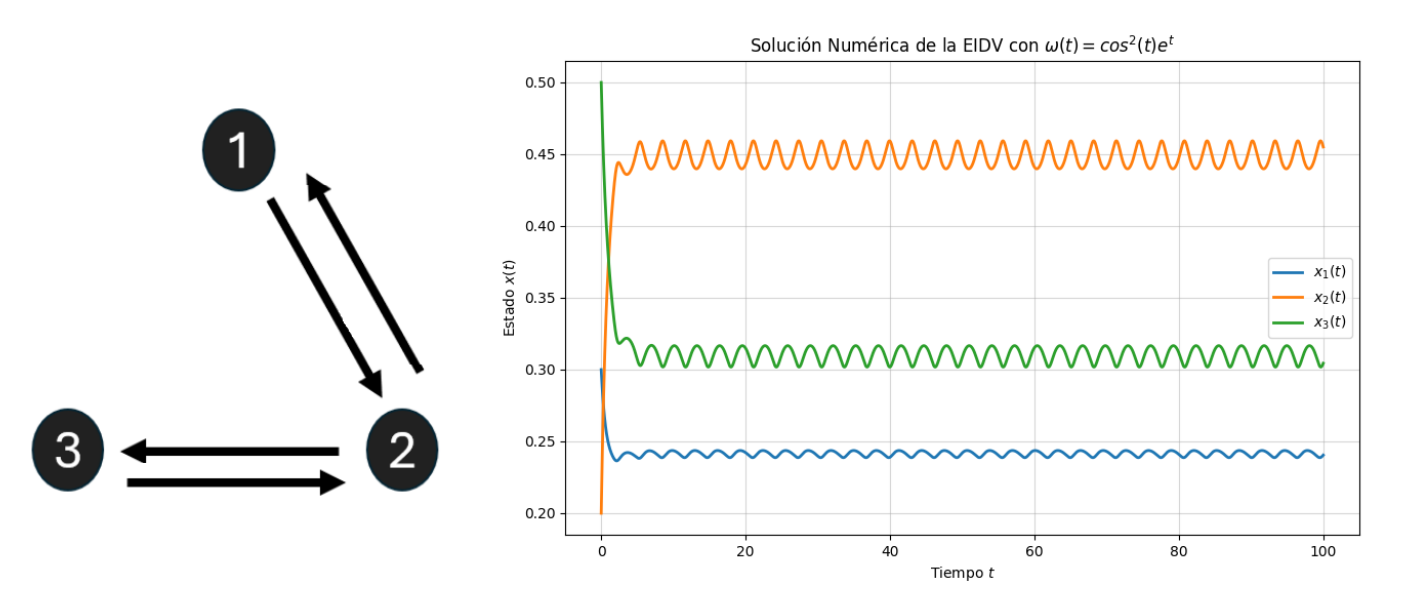
\includegraphics[width=0.82\textwidth]{figures/daniel_rodriguez_luis_fig01_p2_crop.png}

{\small Figura 1. Representación gráfica del sistema dinámico considerado para el vector PageRank con memoria dependiente del tiempo.}
\end{center}


\keywords{sistema dinámico, comportamiento asintótico.}

\begin{multicols}{2}
\begin{enumerate}[label={[\arabic*]},leftmargin=*]
\item D. Aleja, J. Flores, E. Primo, D. Rodríguez, M. Romance, Fixed points of personalized PageRank centrality: From irreducible to reducible networks, \textit{Linear Algebra and its Applications} 733, 233--272 (2026).
\item P. Boldi, M. Santini, S. Vigna, PageRank: Functional dependencies, \textit{ACM Transactions on Information Systems (TOIS)} 27(4) (2009).
\item D. F. Gleich, R. A. Rossi, A dynamical system for pagerank with time-dependent teleportation, \textit{Internet Mathematics} 10, 188--217 (2014).
\item C. D. Meyer, \textit{Matrix Analysis and Applied Linear Algebra}, Society for Industrial and Applied Mathematics, Philadelphia (2000).
\end{enumerate}
\end{multicols}
\end{sincabstract}

% -----------------------------------------------------------------------------
% ABSTRACT 4
% -----------------------------------------------------------------------------
\sincAbstractPage{4}{Propagación no lineal de ultrasonidos en medios viscoelásticos con burbujas: hacia los metamateriales acústicos}

\begin{sincabstract}
{Propagación no lineal de ultrasonidos en medios viscoelásticos con burbujas: hacia los metamateriales acústicos}
{Elena V. Carreras-Casanova, María Teresa Tejedor-Sastre, Christian Vanhille}
{Numerical Analysis in Nonlinear Acoustics Research Group (NANLA), Universidad Rey Juan Carlos (URJC)}
{elena.carreras@urjc.es}

\paragraph{Resumen.}
La presencia de burbujas de gas en un medio modifica radicalmente sus propiedades acústicas. Cerca de su frecuencia de resonancia, actúan como dispersores altamente eficientes, inducen variaciones significativas en la velocidad de propagación e incrementan la atenuación y el comportamiento no lineal. Esta propiedad permite manipular señales acústicas mediante poblaciones de burbujas.

En este trabajo se desarrolla un modelo numérico para la propagación no lineal de ondas ultrasónicas en medios viscoelásticos con burbujas. El modelo acopla la ecuación de onda con una ecuación de Rayleigh--Plesset modificada, que describe la variación del volumen de la burbuja e incorpora la viscoelasticidad del medio mediante el modelo de Kelvin--Voigt [1]. Esta formulación permite estudiar la interacción entre el campo de presión acústica y las oscilaciones de las burbujas, así como la influencia de las propiedades viscoelásticas en la transición entre los regímenes lineal y no lineal [2].

Los resultados numéricos muestran que el módulo elástico del medio reduce la no linealidad, atenúa la generación de armónicos y modifica la estructura espectral de la onda transmitida, mientras que la viscosidad tiene un efecto comparativamente menor. Se analiza también la respuesta acústica de distribuciones no homogéneas de burbujas [3], con especial atención a configuraciones en capas. Se estudia la influencia del tamaño, la densidad y la disposición espacial de las burbujas, así como de la viscoelasticidad del medio, sobre los mecanismos de resonancia y absorción, con vistas al diseño de metamateriales acústicos.

\keywords{acústica no lineal, medios viscoelásticos con burbujas, simulaciones numéricas, dinámica no lineal, metamateriales acústicos.}

\begin{enumerate}[label={[\arabic*]},leftmargin=*]
\item E. V. Carreras-Casanova, C. Vanhille, A Model for the Dynamics of Stable Gas Bubbles in Viscoelastic Fluids Based on Bubble Volume Variation, \textit{Acoustics} 7(4), art. 67 (2025).
\item E. V. Carreras-Casanova, M. T. Tejedor-Sastre, C. Vanhille, Nonlinear propagation of ultrasounds in bubbly viscoelastic media: A study on the influence of the medium properties on the nonlinear parameter, \textit{Ultrasonics Sonochemistry} 122, 107603 (2025).
\item C. Vanhille, Two-Dimensional Numerical Simulations of Ultrasound in Liquids with Gas Bubble Agglomerates: Examples of Bubbly-Liquid-Type Acoustic Metamaterials (BLAMMs), \textit{Sensors} 17(1), 173 (2017).
\end{enumerate}
\end{sincabstract}

% -----------------------------------------------------------------------------
% ABSTRACT 5
% -----------------------------------------------------------------------------
\sincAbstractPage{5}{Conductividad térmica de una cadena de osciladores. El problema de Fermi-Pasta-Ulam-Tsingou}

\begin{sincabstract}
{Conductividad térmica de una cadena de osciladores. El problema de Fermi-Pasta-Ulam-Tsingou}
{Fernán Del Río Martín\textsuperscript{1,2}}
{\textsuperscript{1} Alumno del Máster de Física Avanzada de UNED, Madrid, España\\
\textsuperscript{2} Grupo de Dinámica No Lineal, Caos y Sistemas Complejos, Universidad Rey Juan Carlos, Madrid, España}
{f.delrio.2021@alumnos.urjc.es}

\paragraph{Resumen.}
En este trabajo se estudia la dinámica no lineal y el transporte térmico en cadenas unidimensionales de osciladores tipo Fermi-Pasta-Ulam-Tsingou (FPUT). Como punto de partida, se analiza el fenómeno de recurrencia en el modelo homogéneo, mostrando cómo la energía, inicialmente depositada en el modo espacial fundamental, evade la equipartición térmica de forma inmediata y da lugar a la formación de estructuras coherentes de tipo solitón.

Posteriormente, se investiga el transporte de calor fuera del equilibrio acoplando los extremos de una cadena FPUT-$\beta$ a baños térmicos de Langevin. A partir del cálculo del flujo de calor estacionario y del gradiente térmico interno, se determina la conductividad térmica efectiva del sistema. Para la cadena homogénea, las simulaciones reproducen con éxito los regímenes asintóticos teóricos: $\kappa\sim T^{-1}$ a bajas temperaturas y un escalado de $\kappa\sim T^{1/4}$ en el límite de alta temperatura.

Por último, se evalúa el impacto del desorden estructural mediante la introducción de defectos de masa bajo distintas topologías: un defecto único central, distribución periódica y desorden aleatorio. Se observa que la presencia de estas impurezas reduce significativamente la conductividad térmica efectiva en comparación con el medio homogéneo, actuando como centros de dispersión fonónica que alteran la propagación microscópica de la energía. Notablemente, en el régimen de altas temperaturas, los defectos modifican principalmente el prefactor de la conductividad térmica, preservando un exponente de escalado muy próximo al valor teórico $1/4$ característico del sistema puro.

\keywords{complejidad, dinámica no lineal, FPUT, transporte de calor, conductividad térmica, caos.}
\end{sincabstract}

% -----------------------------------------------------------------------------
% ABSTRACT 6
% -----------------------------------------------------------------------------
\sincAbstractPage{6}{Intermitencia caótica en un láser de clase B con señal inyectada}

\begin{sincabstract}
{Intermitencia caótica en un láser de clase B con señal inyectada}
{Francisco Javier Marín Rodríguez\textsuperscript{1}, Karin Alfaro Bittner\textsuperscript{1}, Jorge Raúl Tredicce\textsuperscript{1}}
{\textsuperscript{1} Departamento de Matemática Aplicada, Universidad Rey Juan Carlos, Móstoles, España}
{javier.marin@urjc.es}

\paragraph{Resumen.}
La intermitencia caótica constituye una de las rutas clásicas al caos en sistemas dinámicos no lineales. Se caracteriza por la alternancia irregular entre fases aparentemente periódicas, llamadas laminares, y episodios de comportamiento desordenado denominados \textit{bursts}. Este fenómeno resulta especialmente interesante porque permite estudiar la transición entre dinámica periódica y dinámica caótica no como un cambio abrupto, sino como un proceso gradual en el que coexisten escalas temporales muy diferentes.

En este trabajo estudiamos la aparición de intermitencia caótica en un láser de clase B sometido a una señal externa inyectada [1]. El modelo normalizado considerado describe la evolución de las dos componentes del campo eléctrico, $x$ e $y$, junto con la inversión de población $z$:
\begin{align*}
\dot{x} &= (z-1)x+(\theta+\delta z)y+A,\\
\dot{y} &= -(\theta+\delta z)x+(z-1)y,\\
\dot{z} &= \frac{\gamma_{\parallel}}{K}\left[-\frac{z(x^2+y^2)}{1+\delta^2}-z+z_0\right].
\end{align*}
Aquí, $A$ representa la amplitud de la señal inyectada; $\theta$ y $\delta$ son el \textit{detuning} de la cavidad y el atómico, respectivamente; $\gamma_{\parallel}$ es la tasa de relajación de la inversión de población; $K$ es la tasa de decaimiento del campo dentro de la cavidad láser (o, equivalentemente, la tasa de pérdida de fotones en la cavidad) y $z_0$ es el bombeo. La intensidad del láser se define como
\begin{equation*}
I(t)=\frac{x^2(t)+y^2(t)}{1+\delta^2}.
\end{equation*}

Realizamos integraciones numéricas del sistema variando los parámetros de control, principalmente la amplitud de inyección $A$ y el \textit{detuning} de la cavidad $\theta$. A partir de la señal de la intensidad $I(t)$, construimos diagramas de bifurcación, distribuciones de longitudes laminares y espectros de Fourier. Estos observables permiten caracterizar la alternancia entre fases laminares y \textit{bursts}, y comparar el comportamiento numérico con los escenarios conocidos de intermitencia caótica [2].

\keywords{intermitencia caótica, láser con señal inyectada, dinámica no lineal, rutas al caos, sistemas complejos.}

\begin{enumerate}[label={[\arabic*]},leftmargin=*]
\item J. R. Tredicce, F. T. Arecchi, G. L. Lippi y G. P. Puccioni, Instabilities in lasers with an injected signal, \textit{Journal of the Optical Society of America B} 2, 173--183 (1985).
\item S. Elaskar, E. del Río y colaboradores, Review of Chaotic Intermittency, \textit{Symmetry} 15, 1195 (2023).
\end{enumerate}
\end{sincabstract}

% -----------------------------------------------------------------------------
% ABSTRACT 7
% -----------------------------------------------------------------------------
\sincAbstractPage{7}{Clasificación de autómatas celulares bajo diferentes condiciones de contorno usando la distancia de Hamming}

\begin{sincabstract}
{Clasificación de autómatas celulares bajo diferentes condiciones de contorno usando la distancia de Hamming}
{Gaspar Alfaro\textsuperscript{1}, Miguel A. F. Sanjuán\textsuperscript{1}}
{\textsuperscript{1} Nonlinear Dynamics, Chaos and Complex Systems Group, Departamento de Física, Universidad Rey Juan Carlos, Tulipán s/n, Móstoles, 28933, Madrid, Spain}
{gaspar.alfaro@urjc.es; miguel.sanjuan@urjc.es}

\paragraph{Resumen.}
Clasificamos los autómatas celulares elementales midiendo la distancia de Hamming de dos configuraciones próximas de cada autómata. Obtenemos series temporales de la distancia que reflejan los comportamientos obtenidos por Wolfram: el comportamiento periódico de la Clase 2 y el caótico de la Clase 3. Finalmente, para la Clase 4, obtenemos series que presentan un transitorio caótico hacia un estado periódico. Este caos transitorio subyace a la transición conocida como \textit{edge of chaos}. Esta manera de clasificar es más fácil de visualizar que simplemente observar los patrones formados por los autómatas celulares.

También comparamos diferentes condiciones de frontera, periódicas o fijas, y descubrimos que el comportamiento de los autómatas varía. Analizando el patrón que forman los autómatas descubrimos que los bordes fijos pueden inducir una periodicidad local en las celdas cercanas al borde. Por lo tanto, para la mayoría de reglas afectadas, el cambio en clasificación es hacia clases con menor complejidad. Aun así, encontramos algunas reglas excepcionales que aumentan su complejidad con fronteras fijas.

\keywords{complejidad, autómatas celulares, distancia de Hamming, condiciones de contorno, patrones de diferencia.}

\begin{enumerate}[label={[\arabic*]},leftmargin=*]
\item S. Wolfram, Universality and complexity in cellular automata, \textit{Physica D} 10, 1 (1984).
\end{enumerate}
\end{sincabstract}

% -----------------------------------------------------------------------------
% ABSTRACT 8
% -----------------------------------------------------------------------------
\sincAbstractPage{8}{Biritmicidad estocástica fuera de la región de coexistencia en el modelo de Hindmarsh-Rose}

\begin{sincabstract}
{Biritmicidad estocástica fuera de la región de coexistencia en el modelo de Hindmarsh-Rose}
{Ignacio Ortega Piwonka\textsuperscript{1}, Javier Used\textsuperscript{1}, Jesús Seoane\textsuperscript{1}, Miguel A. F. Sanjuán\textsuperscript{1,2}}
{\textsuperscript{1} Nonlinear Dynamics, Chaos and Complex Systems Group, Departamento de Física, Universidad Rey Juan Carlos, Tulipán s/n, Móstoles, 28933, Madrid, Spain\\
\textsuperscript{2} Real Academia de Ciencias, Madrid, España}
{Juanignacio.ortega@urjc.es}

\paragraph{Resumen.}
En este trabajo, se demuestra que el modelo de Hindmarsh-Rose sujeto a ruido blanco aditivo exhibe biritmicidad. Específicamente, el sistema fluctúa entre dos atractores con \textit{bursting} caracterizados por un número diferente de picos. Este comportamiento se observa no sólo dentro de la región biestable limitada por dos bifurcaciones de silla-nodo de ciclos límites sino también más allá de las mismas. Este fenómeno está asociado con el efecto fantasma, típicamente observado cerca de bifurcaciones de silla-nodo deterministas. Se ha mapeado la región de biritmicidad estocástica en términos de la intensidad del ruido y un parámetro determinista que controla la dinámica de los canales iónicos rápidos. Con el objeto de proveer un sustento analítico, se presenta un modelo estocástico simple con una sola bifurcación de silla-nodo. En este modelo, la biritmicidad estocástica es caracterizada como una función de la intensidad del ruido y el parámetro de control [1].

\begin{center}
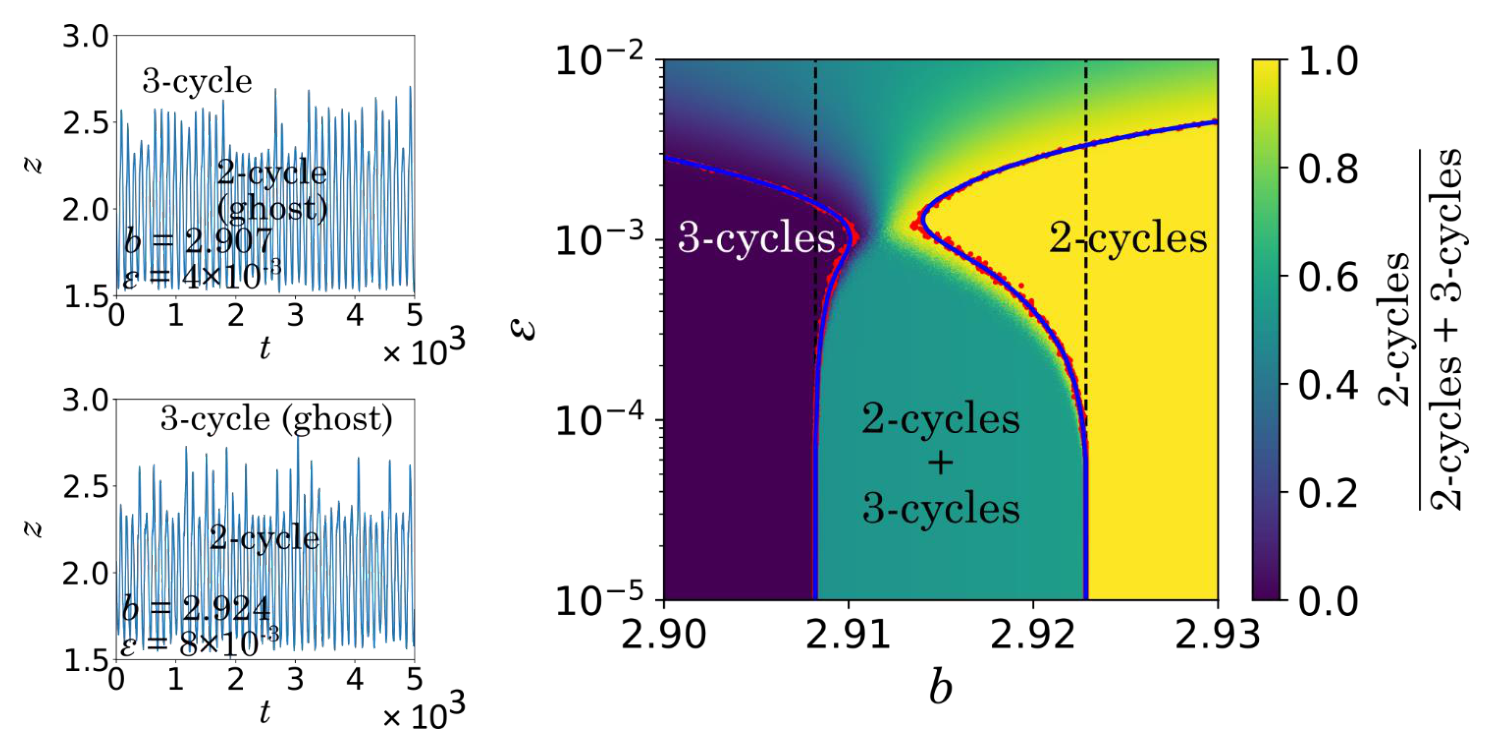
\includegraphics[width=0.82\textwidth]{figures/ignacio_ortega_piwonka_fig01_p1_crop.png}

{\small Figura 1. Dinámica estocástica asociada al modelo de Hindmarsh--Rose en el contexto de la birritmicidad fuera de la región de coexistencia.}
\end{center}

\keywords{modelo neuronal de Hindmarsh-Rose, biritmicidad, fenómeno fantasma, efectos inducidos por ruido.}

\begin{enumerate}[label={[\arabic*]},leftmargin=*]
\item I. Ortega-Piwonka, J. Used, J. M. Seoane, M. A. F. Sanjuán, Stochastic birhythmicity outside the coexistence region in the Hindmarsh-Rose model, \textit{Physical Review E} 111, 044217 (2025).
\end{enumerate}
\end{sincabstract}

% -----------------------------------------------------------------------------
% ABSTRACT 9
% -----------------------------------------------------------------------------
\sincAbstractPage{9}{Término de amortiguamiento fraccionario en osciladores no lineales}

\begin{sincabstract}
{Término de amortiguamiento fraccionario en osciladores no lineales}
{Mattia Coccolo}
{Nonlinear Dynamics, Chaos and Complex Systems Group, Departamento de Física, Universidad Rey Juan Carlos, Tulipán s/n, Móstoles, 28933, Madrid, Spain}
{mattiatommaso.coccolo@urjc.es}

\paragraph{Resumen.}
Esta charla explora los efectos del amortiguamiento fraccionario sobre la dinámica de osciladores no lineales. Utilizando los sistemas de Helmholtz y Duffing como casos de estudio, los resultados presentados muestran cómo la memoria introducida en el término disipativo puede modificar los procesos de escape, la sensibilidad a la fase, el comportamiento asintótico y las propiedades de resonancia. El objetivo principal es mostrar que el amortiguamiento fraccionario no constituye simplemente una generalización de la disipación viscosa estándar, sino un mecanismo dinámico genuino capaz de producir comportamientos cualitativamente nuevos.

La charla se basa en varios trabajos recientes sobre amortiguamiento fraccionario en osciladores de Helmholtz y Duffing.

\keywords{amortiguamiento fraccionario, osciladores no lineales, memoria, Duffing, Helmholtz, resonancia.}

\begin{enumerate}[label={[\arabic*]},leftmargin=*]
\item M. Coccolo, J. M. Seoane, M. A. F. Sanjuán, Fractional damping induces resonant behavior in the Duffing oscillator, \textit{Communications in Nonlinear Science and Numerical Simulation} 133, 107965.
\item M. Coccolo, J. M. Seoane, S. Lenci, M. A. F. Sanjuán, Fractional damping effects on the transient dynamics of the Duffing oscillator, \textit{Communications in Nonlinear Science and Numerical Simulation} 117, 106959.
\item A. Ortiz, J. Yang, M. Coccolo, J. M. Seoane, M. A. F. Sanjuán, Fractional damping enhances chaos in the nonlinear Helmholtz oscillator, \textit{Nonlinear Dynamics} 102(4), 2323--2337.
\item M. Coccolo, J. M. Seoane, S. Lenci, M. A. F. Sanjuán, Phase control of escapes in the fractional damped Helmholtz oscillator, \textit{Chaos, Solitons \& Fractals} 183, 114918.
\end{enumerate}
\end{sincabstract}

% -----------------------------------------------------------------------------
% ABSTRACT 10
% -----------------------------------------------------------------------------


\sincAbstractPage{10}{Diferenciación ontológica y navegación semántica en redes léxicas}

\begin{sincabstract}
{Diferenciación ontológica y navegación semántica en redes léxicas}
{Pablo García}
{Complex Systems Group, Universidad Politécnica de Madrid, Madrid, Spain}
{pablo.garcia.cuadrillero@upm.es}

\paragraph{Resumen.}
Comprender las relaciones semánticas dentro de redes complejas derivadas de recursos léxicos es fundamental para la ciencia de redes y el modelado del lenguaje. Aunque los métodos de incrustación de redes, o \textit{network embedding}, capturan la similitud contextual, cuantificar la distancia semántica basándose directamente en la estructura definicional explícita sigue siendo un desafío. Las medidas precisas de similitud semántica permiten la navegación en redes léxicas basada en maximizar la similitud semántica en cada salto de navegación, lo que denominamos navegación semántica, o \textit{Semantic Navigation} (SN).

Este trabajo introduce la diferenciación ontológica, u \textit{Ontological Differentiation} (OD), un método formal para medir la divergencia entre conceptos mediante el análisis de las coincidencias que aparecen durante la expansión recursiva de definiciones. La metodología se aplica a redes extraídas del \textit{Simple English Wiktionary}, comparando las puntuaciones de OD con otras medidas de similitud semántica propuestas en la literatura, en particular la similitud coseno basada en la exploración de redes mediante recorridos aleatorios.

Encontramos correlaciones débiles entre las puntuaciones OD directas por pares y las similitudes coseno a lo largo de aproximadamente dos millones de pares de palabras, muestreados de un conjunto que representa más del 50\,\% de las entradas del léxico de Wiktionary. Esto establece a OD como una métrica semántica basada en definiciones y en gran medida independiente, cuya ortogonalidad respecto a la similitud coseno se vuelve más pronunciada cuando se eliminan del conjunto de datos los términos con bajo contenido semántico.

Además, utilizamos puntuaciones OD acumuladas para evaluar trayectorias generadas tanto por la SN basada en vectores como por los caminos más cortos, o \textit{Shortest Paths} (SP), estructuralmente óptimos a través de las redes. Encontramos que las trayectorias SN presentan de forma consistente puntuaciones OD acumuladas significativamente menores que los caminos más cortos, lo que sugiere que la SN produce recorridos más coherentes con la estructura definicional del diccionario, según la medida proporcionada por OD.

La diferenciación ontológica proporciona así una nueva herramienta, fundamentada en definiciones, para analizar la estructura semántica y validar procesos de navegación en redes léxicas.

\keywords{redes léxicas, diferenciación ontológica, navegación semántica, similitud semántica, Wiktionary, ciencia de redes.}

\end{sincabstract}




% -----------------------------------------------------------------------------
% ABSTRACT 11
% -----------------------------------------------------------------------------
\sincAbstractPage{11}{Dinámica de solitones en generalizaciones complejas de la ecuación de mKdV}

\begin{sincabstract}
{Dinámica de solitones en generalizaciones complejas de la ecuación de mKdV}
{Paz Albares Vicente}
{Departamento de Matemática Aplicada a la Ingeniería Industrial, Universidad Politécnica de Madrid, 28012 Madrid, Spain}
{paz.albares@upm.es}

\paragraph{Resumen.}
Las ecuaciones de Korteweg--de Vries (KdV) y de Schrödinger no lineal (NLS) constituyen dos de los modelos fundamentales en la teoría de solitones y sistemas integrables. Ambas ecuaciones aparecen en la descripción de fenómenos no lineales en diversos contextos, como óptica no lineal, dinámica de fluidos o física de la materia condensada. Desde el punto de vista matemático, comparten una rica estructura asociada a la integrabilidad, como la existencia de pares de Lax, infinitas cantidades conservadas y una compleja geometría subyacente que permite caracterizar completamente su dinámica.

La ecuación modificada de Korteweg--de Vries (mKdV) surge como una extensión natural de la ecuación de KdV y hereda muchas de sus propiedades integrables. En esta charla se presentan distintas generalizaciones complejas de la ecuación de mKdV. La caracterización de su integrabilidad y soluciones se aborda mediante el análisis de Painlevé, el método de la variedad singular y transformaciones binarias de Darboux. La combinación de estas técnicas permite obtener el problema espectral asociado y familias de soluciones exactas. En particular, se estudia en detalle la dinámica y las propiedades de diferentes configuraciones solitónicas. Mientras que en el caso real aparecen esencialmente soluciones de solitones de línea (solitones clásicos de KdV), la extensión compleja del modelo da lugar a estructuras racionales de tipo \textit{rogue wave}, soluciones características de la ecuación de NLS.

Estos resultados se enmarcan en trabajos en colaboración con P. G. Estévez, A. González-Parra y P. del Olmo [1,2].

\keywords{integrabilidad, problema espectral, dinámica no lineal, solitones.}

\begin{enumerate}[label={[\arabic*]},leftmargin=*]
\item P. Albares y P. G. Estévez, A Comprehensive Study of the Complex mKdV Equation through the Singular Manifold Method, \textit{Mathematics} 11, 859 (2023).
\item P. Albares, P. G. Estévez, A. González-Parra y P. del Olmo, Spectral problem for the complex mKdV equation: singular manifold method and Lie symmetries, \textit{Open Communications in Nonlinear Mathematical Physics}, Special Issue in Memory of Decio Levi 1, 1 (2024).
\end{enumerate}
\end{sincabstract}

% -----------------------------------------------------------------------------
% ABSTRACT 12
% -----------------------------------------------------------------------------
\sincAbstractPage{12}{Resiliencia inducida por dispersión a fluctuaciones ambientales estocásticas en poblaciones con efecto Allee}

\begin{sincabstract}
{Resiliencia inducida por dispersión a fluctuaciones ambientales estocásticas en poblaciones con efecto Allee}
{Rodrigo Crespo Miguel\textsuperscript{1,2}, Javier Jarillo Díaz\textsuperscript{3,4}, Francisco J. Cao García\textsuperscript{2,5}}
{\textsuperscript{1} Departamento de Geología, Física y Química Inorgánica, Universidad Rey Juan Carlos, Móstoles, España\\
\textsuperscript{2} Departamento de Estructura de la Materia, Física Térmica y Electrónica, Facultad de Ciencias Físicas, Universidad Complutense de Madrid, Madrid, España\\
\textsuperscript{3} Departamento de Estadística e Investigación Operativa, Facultad de Ciencias Físicas, Universidad Complutense de Madrid, Madrid, España\\
\textsuperscript{4} Research Unit of Environmental and Evolutionary Biology, Namur Institute of Complex Systems, and Institute of Life, Earth, and the Environment, Universidad de Namur, Namur, Bélgica\\
\textsuperscript{5} Instituto Madrileño de Estudios Avanzados en Nanociencia (IMDEA-Nanociencia), Madrid, España}
{rodrigo.crespom@urjc.es}

\paragraph{Resumen.}
Muchas especies son insostenibles a densidades de población bajas (efecto Allee). Por debajo del llamado umbral de Allee, la población disminuye en lugar de crecer. Aunque en una población local cerrada las fluctuaciones ambientales siempre conducen a la extinción, la dispersión puede conducir a regiones con población sostenible, siempre que la amplitud de las fluctuaciones ambientales esté por debajo de un umbral de extinción. Hemos identificado dos tipos de poblaciones sostenibles: poblaciones de alta densidad y poblaciones de baja densidad. Nuestros resultados muestran que los puntos donde la población es alta, baja o extinta coexisten cuando la población está cerca de la extinción global (incluso para hábitats homogéneos). El umbral de extinción es máximo para distancias de dispersión características mucho mayores que la escala de correlación espacial de las fluctuaciones ambientales. El umbral de extinción aumenta proporcionalmente a la raíz cuadrada de la tasa de dispersión y disminuye con el umbral de Allee. Este marco teórico proporciona un enfoque único para abordar otros factores, como la fragmentación del hábitat o la recolección, que afectan a la resiliencia de la población ante las fluctuaciones ambientales.

\keywords{dinámica no lineal, dinámica de poblaciones, ecología, mecánica estadística del no equilibrio.}

\begin{enumerate}[label={[\arabic*]},leftmargin=*]
\item R. Crespo-Miguel, J. Jarillo, F. J. Cao-García, Dispersal-induced resilience to stochastic environmental fluctuations in populations with Allee effect, \textit{Physical Review E} 105, 014413 (2022).
\end{enumerate}
\end{sincabstract}

% -----------------------------------------------------------------------------
% ABSTRACT 13
% -----------------------------------------------------------------------------
\sincAbstractPage{13}{Eficiencia termodinámica de estructuras disipativas acopladas}

\begin{sincabstract}
{Eficiencia termodinámica de estructuras disipativas acopladas}
{Álvaro García López\textsuperscript{1}, Inés Pérez Mariño\textsuperscript{1}, Alfonso Delgado-Bonal}
{\textsuperscript{1} Nonlinear Dynamics, Chaos and Complex Systems Group, Departamento de Física, Universidad Rey Juan Carlos, Tulipán s/n, Móstoles, 28933, Madrid, Spain}
{alvaro.lopez@urjc.es}

\vspace{-0.5cm}

\paragraph{Resumen.}
Las estructuras disipativas son sistemas dinámicos abiertos que mantienen una organización coherente mediante el intercambio continuo de energía y materia con el entorno y la generación de entropía [1]. Un análisis reciente de la rueda hidráulica de Malkus--Lorenz interpretó el sistema de Lorenz como una máquina térmica y mostró que su eficiencia aumenta al alejarse del equilibrio, aunque presenta caídas pronunciadas cerca de la transición al caos [2]. En este trabajo se extiende ese enfoque a estructuras disipativas acopladas. Para ello, se estudian dos tipos de acoplamiento ---maestro-esclavo y difusivo simétrico--- y se demuestran leyes que permiten describir los sistemas compuestos como una única máquina equivalente con una eficiencia bien definida. Aplicando estos resultados a ruedas hidráulicas de Lorenz acopladas, se obtienen fórmulas de eficiencia coherentes con el balance energético del sistema [3]. Las simulaciones numéricas muestran que el acoplamiento en serie tiende a aumentar la eficiencia termodinámica, mientras que el acoplamiento en paralelo incrementa el flujo total de energía y promedia la eficiencia de los sistemas. Además, la sincronización suele ser neutra o favorable para la eficiencia, salvo en regiones muy específicas de parámetros, y el acoplamiento altera los patrones de generación de entropía. En conjunto, los resultados proponen un marco matemáticamente riguroso y transparente para definir y calcular la eficiencia termodinámica en redes de flujo complejas, con posibles aplicaciones al estudio energético de sistemas complejos.

\begin{center}
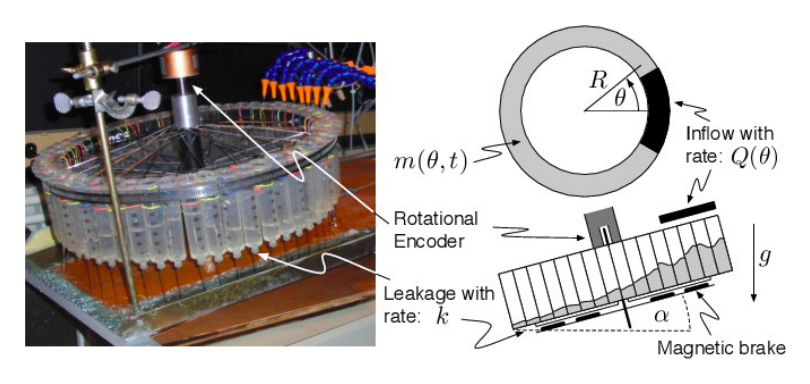
\includegraphics[width=0.66\textwidth]{figures/alvaro_garcia_fig01_p1_crop.png}

\vspace{-0.7em}
{\small Figura 1. Esquema de estructuras disipativas acopladas y eficiencia termodinámica.}
\end{center}

\vspace{-0.6em}

\keywords{estructuras disipativas, ruptura de la simetría, autooscilaciones, eficiencia termodinámica, sistema de Lorenz, sistemas fuera del equilibrio.}

\vspace{-0.4em}

\begin{multicols}{2}

{\small
\begin{enumerate}[label={[\arabic*]},leftmargin=*,itemsep=0.15em,topsep=0.2em]
\item I. Prigogine, R. Lefever, Symmetry breaking instabilities in dissipative systems, \textit{Journal of Chemical Physics} 48, 1695 (1968).

\item Á. G. López, F. Benito, J. Sabuco, A. Delgado-Bonal, The thermodynamic efficiency of the Lorenz system, \textit{Chaos, Solitons \& Fractals} 172, 113521 (2023).

\item Á. G. López, P. I. Mariño, A. Delgado-Bonal, The thermodynamic efficiency of coupled dissipative structures, arXiv:2604.16549 (2026).
\end{enumerate}
}
\end{multicols}
\end{sincabstract}

\clearpage
\phantomsection
\label{sec:temas}
\addcontentsline{toc}{section}{Temas tratados}
\begin{center}
\section*{\Huge Temas tratados}
\end{center}
\vspace{0.8em}

Las contribuciones recogidas en este libro reflejan la diversidad de enfoques científicos presentes en SINC II. A continuación se ofrece un índice temático orientativo, pensado como guía de lectura y como ayuda para identificar posibles puntos de conexión entre las distintas comunicaciones.

\begin{itemize}[leftmargin=*]

    \item \textbf{Sistemas dinámicos, no linealidad y complejidad}
    \begin{itemize}
        \item Sistemas de EDOs polinómicas.
        \item Osciladores no lineales con amortiguamiento fraccionario.
        \item Intermitencia caótica en láseres.
        \item Dinámica de solitones en ecuaciones no lineales.
        \item Birritmicidad estocástica en modelos neuronales.
    \end{itemize}

    \item \textbf{Redes complejas, navegación y estructura semántica}
    \begin{itemize}
        \item Dinámica del vector PageRank con memoria dependiente del tiempo.
        \item Clasificación de autómatas celulares mediante distancia de Hamming.
        \item Navegación semántica y diferenciación ontológica en redes léxicas.
    \end{itemize}

    \item \textbf{Física estadística, transporte y termodinámica}
    \begin{itemize}
        \item Conductividad térmica en cadenas de osciladores.
        \item Problema de Fermi--Pasta--Ulam--Tsingou.
        \item Eficiencia termodinámica de estructuras disipativas acopladas.
    \end{itemize}

    \item \textbf{Biología, astrobiología y evolución}
    \begin{itemize}
        \item Polimerización, replicación y evolución del ARN en el origen de la vida.
        \item Evolución prebiótica y complejidad molecular.
        \item Dinámica de poblaciones con efecto Allee bajo fluctuaciones estocásticas.
    \end{itemize}

    \item \textbf{Ondas, medios complejos y metamateriales}
    \begin{itemize}
        \item Propagación no lineal de ultrasonidos en medios viscoelásticos con burbujas.
        \item Metamateriales acústicos.
    \end{itemize}

    \item \textbf{Métodos matemáticos y computacionales}
    \begin{itemize}
        \item Álgebra conmutativa y álgebra real aplicadas a sistemas dinámicos.
        \item Modelización computacional de procesos físico-químicos y biológicos.
        \item Simulación, análisis de redes y métricas de similitud.
    \end{itemize}

\end{itemize}

Este índice no pretende establecer una clasificación cerrada de las contribuciones, sino destacar algunas de las líneas transversales que atraviesan el simposio y que pueden servir como punto de partida para nuevas discusiones y colaboraciones.



% ============================================================
% PARTICIPANTES Y ORGANIZACIÓN
% Añadir al final del documento, antes de \end{document}
% ============================================================

\clearpage
\phantomsection
\label{sec:ponentes}
\addcontentsline{toc}{section}{Ponentes}

\begin{center}
{\LARGE\bfseries Ponentes}
\end{center}

\vspace{0.5cm}

\small

\begin{description}[style=multiline,leftmargin=4.3cm,font=\normalfont\bfseries]

\item[Alexandru Iosif]
Área de Matemática Aplicada, Universidad Rey Juan Carlos, Madrid, España.\\
\href{mailto:alexandru.iosif@urjc.es}{alexandru.iosif@urjc.es}

\item[Carla Alejandre]
Centro de Astrobiología (CAB), CSIC--INTA, Torrejón de Ardoz, Madrid, España;
Grupo Interdisciplinar de Sistemas Complejos (GISC), Madrid, España.\\
\href{mailto:calejandre@cab.inta-csic.es}{calejandre@cab.inta-csic.es}

\item[Daniel José Rodríguez Luis]
Universidad Rey Juan Carlos, Madrid, España.\\
\href{mailto:danieljose.rodriguez@urjc.es}{danieljose.rodriguez@urjc.es}

\item[Elena V. Carreras-Casanova]
Numerical Analysis in Nonlinear Acoustics Research Group (NANLA),
Universidad Rey Juan Carlos, Madrid, España.\\
\href{mailto:elena.carreras@urjc.es}{elena.carreras@urjc.es}

\item[Fernán del Río Martín]
Máster Universitario en Física Avanzada, Universidad Nacional de Educación
a Distancia; Grupo de Dinámica No Lineal, Caos y Sistemas Complejos,
Universidad Rey Juan Carlos, Madrid, España.\\
\href{mailto:f.delrio.2021@alumnos.urjc.es}
{f.delrio.2021@alumnos.urjc.es}

\item[Francisco Javier Marín Rodríguez]
Departamento de Matemática Aplicada, Universidad Rey Juan Carlos,
Campus de Móstoles, Madrid, España.\\
\href{mailto:javier.marin@urjc.es}{javier.marin@urjc.es}

\item[Gaspar Alfaro]
Grupo de Dinámica No Lineal, Caos y Sistemas Complejos,
Universidad Rey Juan Carlos, Campus de Móstoles, Madrid, España.\\
\href{mailto:gaspar.alfaro@urjc.es}{gaspar.alfaro@urjc.es}

\item[Ignacio Ortega Piwonka]
Grupo de Dinámica No Lineal, Caos y Sistemas Complejos,
Universidad Rey Juan Carlos, Campus de Móstoles, Madrid, España.\\
\href{mailto:juanignacio.ortega@urjc.es}{juanignacio.ortega@urjc.es}

\item[Mattia Coccolo]
Departamento de Geología, Física y Química Inorgánica,
Universidad Rey Juan Carlos, Campus de Móstoles, Madrid, España.\\
\href{mailto:mattiatommaso.coccolo@urjc.es}
{mattiatommaso.coccolo@urjc.es}

\item[Pablo García]
Complex Systems Group, Universidad Politécnica de Madrid, Madrid, España.\\
\href{mailto:pablo.garcia.cuadrillero@upm.es}
{pablo.garcia.cuadrillero@upm.es}

\item[Paz Albares Vicente]
Departamento de Matemática Aplicada a la Ingeniería Industrial,
Universidad Politécnica de Madrid, Madrid, España.\\
\href{mailto:paz.albares@upm.es}{paz.albares@upm.es}

\item[Rodrigo Crespo Miguel]
Departamento de Geología, Física y Química Inorgánica,
Universidad Rey Juan Carlos, Campus de Móstoles, Madrid, España;
Departamento de Estructura de la Materia, Física Térmica y Electrónica,
Universidad Complutense de Madrid, Madrid, España.\\
\href{mailto:rodrigo.crespom@urjc.es}{rodrigo.crespom@urjc.es}

\item[Álvaro García López]
Departamento de Geología, Física y Química Inorgánica,
Universidad Rey Juan Carlos, Campus de Móstoles, Madrid, España.\\
\href{mailto:alvaro.lopez@urjc.es}{alvaro.lopez@urjc.es}

\end{description}

\normalsize
% ============================================================
% OTROS PARTICIPANTES
% ============================================================
\newpage
%\clearpage
%\phantomsection
%\label{sec:otros-participantes}
%\addcontentsline{toc}{section}{Otros participantes}

\begin{center}
{\LARGE\bfseries Otros participantes}
\end{center}

\vspace{0.6cm}

\small

\noindent
\textbf{Fernando Arias Aragón}\\
Universidad Rey Juan Carlos, Madrid, España.\\
\href{mailto:fernando.arias@urjc.es}
     {fernando.arias@urjc.es}

\medskip

\noindent
\textbf{Natalia Montero San José}\\
Universidad Autónoma de Madrid, Madrid, España.\\
\href{mailto:nmonterosanjose@gmail.com}
     {nmonterosanjose@gmail.com}

\medskip

\noindent
\textbf{Adolfo Alsina}\\
Universidad Rey Juan Carlos, Madrid, España.\\
\href{mailto:adolfo.alsina@urjc.es}
     {adolfo.alsina@urjc.es}

\medskip

\noindent
\textbf{Paula Rodríguez Sánchez}\\
Universidad Rey Juan Carlos, Madrid, España.\\
\href{mailto:paula.rodriguez@urjc.es}
     {paula.rodriguez@urjc.es}

\medskip

\noindent
\textbf{Julieta Schwartz}\\
Universidad Rey Juan Carlos, Madrid, España.\\
\href{mailto:schwartz.julieta@gmail.com}
     {schwartz.julieta@gmail.com}

\medskip

\noindent
\textbf{Sergio Salazar}\\
Universidad Rey Juan Carlos, Madrid, España.\\
\href{mailto:sergio.salazar@urjc.es}
     {sergio.salazar@urjc.es}

\medskip

\noindent
\textbf{Karin Alfaro}\\
Universidad Rey Juan Carlos, Madrid, España.\\
\href{mailto:karin.alfaro@urjc.es}
     {karin.alfaro@urjc.es}

\medskip

\noindent
\textbf{Alexandre Wagemakers}\\
Universidad Rey Juan Carlos, Madrid, España.\\
\href{mailto:alexandre.wagemakers@urjc.es}
     {alexandre.wagemakers@urjc.es}

\medskip

\noindent
\textbf{Teodor A. Diaconescu}\\
Universidad Rey Juan Carlos, Madrid, España.\\
\href{mailto:teodor.diaconescu@urjc.es}
     {teodor.diaconescu@urjc.es}

\normalsize


\clearpage
\phantomsection
\label{sec:comite}
\addcontentsline{toc}{section}{Comité organizador}

\begin{center}
{\LARGE\bfseries Comité organizador}
\end{center}

\vspace{0.5cm}

\noindent
Todos los miembros del comité organizador están afiliados al
\emph{Departamento de Geología, Física y Química Inorgánica,
Universidad Rey Juan Carlos, Campus de Móstoles, Madrid, España}.

\vspace{0.8cm}

\small

\noindent
\textbf{Mattia Coccolo}\\
\href{mailto:mattiatommaso.coccolo@urjc.es}
     {mattiatommaso.coccolo@urjc.es}

\medskip

\noindent
\textbf{Álvar Daza Esteban}\\
\href{mailto:alvar.daza@urjc.es}
     {alvar.daza@urjc.es}

\medskip

\noindent
\textbf{Álvaro García López}\\
\href{mailto:alvaro.lopez@urjc.es}
     {alvaro.lopez@urjc.es}

\medskip

\noindent
\textbf{Rubén Capeáns Rivas}\\
\href{mailto:ruben.capeans@urjc.es}
     {ruben.capeans@urjc.es}

\medskip

\noindent
\textbf{Oibar Martínez Vílchez}\\
\href{mailto:oibar.vilchez@urjc.es}
     {oibar.vilchez@urjc.es}

\medskip

\noindent
\textbf{Andrea Vioque Rodríguez}\\
\href{mailto:andrea.vioque@urjc.es}
     {andrea.vioque@urjc.es}

\medskip

\noindent
\textbf{Miguel Ángel Prado Reynoso}\\
\href{mailto:miguelangel.prado@urjc.es}
     {miguelangel.prado@urjc.es}

\medskip

\noindent
\textbf{Rubén Cabrero Molina}\\
\href{mailto:r.cabrero.2022@alumnos.urjc.es}
     {r.cabrero.2022@alumnos.urjc.es}

\normalsize






\end{document}
